% ============================================================
\chapter{A3: Decomposing the Gain}
\label{chap:evaluation}
% ============================================================

This chapter evaluates (A3, addressing C3). Its structure follows the
logical order in which the research question must be answered. Section~\ref{sec:method} fixes
how the gain is measured. Section~\ref{sec:r1} tests Requirement 1,
whether the causal graph improves on the correlation matrix at all, and
disposes of the driver route the project began from.
Section~\ref{sec:decomposition} presents the decomposition of the gain
into
skeleton and orientation (the answer to the research question), together with its
robustness to the design's free parameters. Section~\ref{sec:believe-rigour}
subjects every claim to the multiplicity-aware inference battery, and
Section~\ref{sec:believe} closes with the threats to validity.

\section{Measurement protocol}
\label{sec:method}

\paragraph{Protocol.} Every configuration runs the identical walk-forward
backtest: the fixed 99-name universe, monthly rebalancing over 2007--2024
(215 rebalances at windows up to one year; the 18-month and two-year
windows' longer burn-ins leave 209 and 203), estimation windows of 189, 252,
378 and 504 trading days for both the graph fit and the sample covariance,
weights held for 21 trading days, transaction costs of 5\,bps per unit of
one-way turnover (swept over $\{0,5,10,20\}$\,bps). ``Performance'' always means the \emph{out-of-sample,
net-of-cost, annualised Sharpe ratio of daily portfolio returns}, reported
alongside CAGR, maximum drawdown and mean turnover
(Table~\ref{tab:return-terms} in Appendix~\ref{app:tables} tabulates them
for the headline
configurations); no in-sample number appears anywhere in this report, and
gross figures appear only as the zero-cost arm of the cost sweep.

\paragraph{Inference.} Pairwise contrasts use the Politis--Romano stationary
block bootstrap \cite{politis1994stationary} (10{,}000 resamples, mean
block 21
days), which resamples the joint return panel so cross-strategy correlation
is preserved. Because daily returns here are heavily non-normal (excess
kurtosis ${\approx}\,\rsKurtosis$; Figure~\ref{fig:retdist}) and because this
project evaluated \rsNtrials\ configurations in total (the deflation
universe deliberately keeps byte-identical duplicates, a conservative
choice), pairwise
$p$-values are never taken at face value: every claim is re-adjudicated by
the battery of Section~\ref{sec:believe-rigour}: Probabilistic and
Deflated Sharpe ratios \cite{bailey2012psr,bailey2014deflated} (the DSR
deflating against all \rsNtrials\ trials), White's Reality Check
\cite{white2000reality}, Hansen's SPA \cite{hansen2005spa} for each
family-wise comparison, and the $90\%$ Model Confidence Set
\cite{hansen2011mcs}. Regimes are defined by NBER recession dates and
top/bottom VIX quintiles.

\paragraph{Stability.} Two further checks target the failure modes of the
incumbent framework specifically. The \emph{seed audit} re-runs the complete
driver-route pipeline under \rsSeedN\ different neural-network seeds with
everything else frozen, measuring how much of its performance is
initialisation noise (Section~\ref{sec:seed-audit}); the graph-based
allocators need no
such audit, being deterministic, a
property verified by the replication gate
(Section~\ref{sec:ablation-design}). Every number in this chapter comes
from the pipeline of Section~\ref{sec:cache}.

\begin{figure}[tbp]
  \centering
  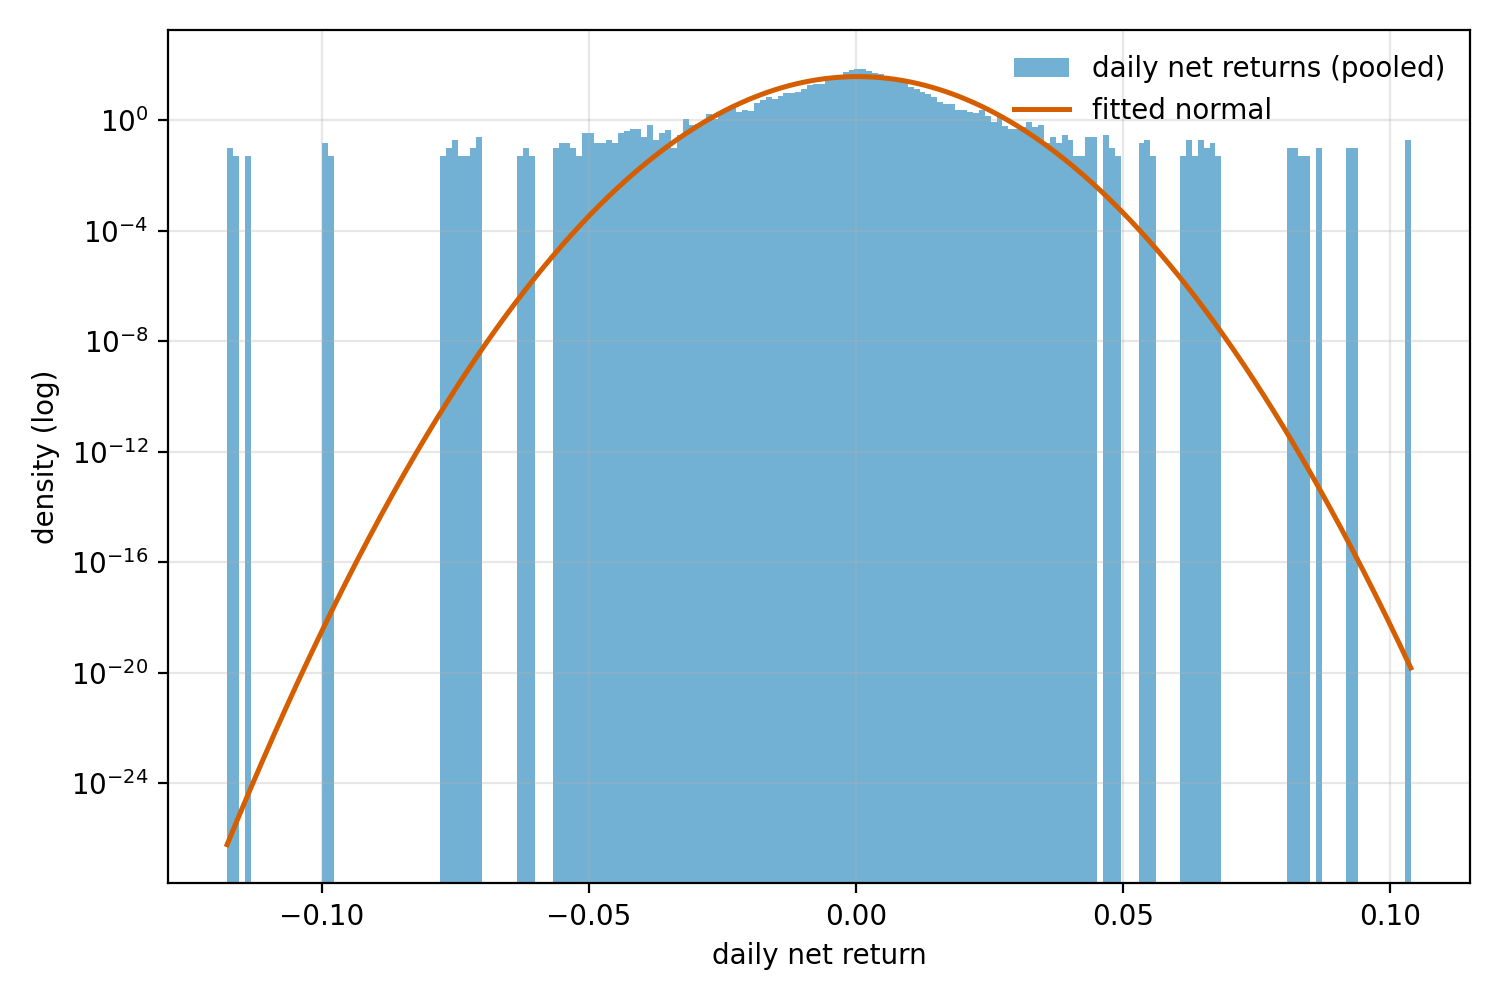
\includegraphics[width=0.7\textwidth]{figures/returns_distribution.png}
  \caption{Distribution of daily net returns (pooled across variants) against
    a fitted normal, log-density axis. The heavy tails (excess kurtosis
    ${\approx}\,\rsKurtosis$) are why the plain Sharpe ratio is supplemented
    by the Probabilistic and Deflated Sharpe ratios throughout.}
  \label{fig:retdist}
\end{figure}

\section{Requirement 1: the causal graph against the correlation matrix}
\label{sec:r1}

Requirement 1 asks whether there is any gain to decompose. The like-for-like
comparison is the graph-blind \HRP{} control against the causal-graph
allocators on the same machinery, at all four windows. The control itself
earns $\rsCorrSharpeWone$, $\rsCorrSharpe$, $\rsCorrSharpeWthree$ and
$\rsCorrSharpeWfive$ at the 189-, 252-, 378- and 504-day windows; the
decomposition's reference treatment (\skelsem{}, which differs from the
skeleton control in the allocation step alone) delivers a total
causal-graph gain over it of $+0.018$,
$+0.031$, $+0.030$ and $+0.032$ respectively ($p=0.43$--$0.11$;
Table~\ref{tab:decomp}), with \orientsem{} reaching $+0.036$ at two
years. Of the 40
graph-versus-\HRP{} cells (five graph-consuming allocators, both
discovery methods, four windows), 36 are above the control (19 of 20 under
DYNOTEARS; the single exception is the skeleton-only allocator at the
nine-month window). This consistency should be read as robustness, not as
significance: the cells share one return panel, overlapping windows and
common machinery, so they are far from independent draws and no sign-count
converts into a valid $p$-value. What it establishes is that the gain's
direction does not depend on the choice of allocator, discovery method or
window; no cell is individually significant, and inference under the
panel's dependence structure is delegated to the family-wise test.
Hansen's SPA over the full allocator grid gives
$p=\rsSpaSkelWonePre$, $\rsSpaSkelWtwoPre$, $\rsSpaSkelWthreePre$ and
$\rsSpaSkelWfivePre$ across the four windows: no rejection anywhere.
Over the narrowed family the report defines, a restriction fixed only
after these results were seen (Section~\ref{sec:believe-rigour}), the
same test gives $p=\rsSpaSkelWone$, $\rsSpaSkelWtwo$,
$\rsSpaSkelWthree$ and $\rsSpaSkelWfive$, crossing the $5\%$ bar at the
two longest windows. Requirement 1 therefore rests on the sign
consistency and the stable total, not on family-wise significance: the
causal graph out-performs the correlation matrix by a modest margin at
every window. The narrowed-family rejections at 18 months and two
years add suggestive, not confirmatory, support, at a size
Section~\ref{sec:believe-rigour} weighs. The decomposition that follows
does not stand or fall with Requirement 1 in any case: it compares the
graph-fed allocators against each other on identical inputs, so it
remains informative about where any gain, whatever its size, comes
from. In return
terms the gain is $+0.4$ to $+0.7$ percentage points of net CAGR per year
($5.62\%$ vs $4.97\%$ for \skelsem{} against the control at one year;
Table~\ref{tab:return-terms}). Two naive anchors bound the absolute
levels: equal weight earns $\rsEwSharpe$ and inverse variance
$\rsIvpSharpe$ at one year (Table~\ref{tab:return-terms}), so every
member of the hierarchical family clears $1/N$ at every window, though
the correlation control itself trails inverse variance at three of the
four windows. The
thesis's claims are contrasts within the family; the anchors size the
family's absolute edge on this universe as modest.

Two contextual facts inform this reading. First, an earlier phase of this
project reported the same comparison against \hspbase{}
(correlation-selected drivers plus neural sensitivities) and found it
strongly significant ($+0.032$, $p<0.001$; family-wise
$p=\rsSpaConsistent$). The \HRP{} control explains the discrepancy:
plain correlation-distance HRP itself beats \hspbase{} ($\rsCorrSharpe$ vs $0.371$
at
one year), so the HSP driver-and-network machinery subtracts value
relative to textbook HRP, and much of the earlier significance was a
statement about \hspbase{}'s machinery rather than about the correlation matrix.
Stating the question
against the stronger control is the more conservative choice, and it
costs the headline its stars.

\paragraph{The driver route is a documented dead end.} The rest of this
section disposes of the arm the project began from, because its failure
motivates allocating from the graph directly. Causal driver selection
(\hspcausal{})
beats \hspbase{} at the data-chosen $K{=}17$ ($+0.010$, $p=0.27$) and
marginally at $K{=}14$ ($+0.003$, $p=0.77$), but trails it at $K=10$, $20$
and $25$ ($-0.015$, $-0.016$, $-0.010$), so the sign of the difference
depends on a parameter the data chose (Figure~\ref{fig:ksens}). No
difference at any $K$ is significant ($p=0.10$--$0.77$). The edge is
therefore
$K$-fragile, consistent with the calibration finding that zero drivers
clear
FDR-controlled significance (Section~\ref{sec:selection}). The closed loop
(\hsploop{}) is exactly inert: across the full
$\alpha\in\{0.4,0.6,0.8\}\times\gamma\in\{0.1,0.3,0.5\}$ grid its weights
equal open-loop \hspcausal{}'s at every rebalance (Figure~\ref{fig:grid}),
because the
utility blend can only re-rank drivers within the causally-selected
set. Even where it could act, it could not learn: the monthly reward
$R[t]$ is a Sharpe ratio estimated from 21 daily observations, and across
215
rebalances it has mean $\rsRewardMean$ and standard deviation
$\rsRewardStd$, a per-update signal-to-noise ratio of
${\approx}\,\rsRewardSNR$. The update frequency is itself the measurement
problem: a monthly loop receives one number a month that is ${\sim}95\%$
noise, so no feedback rule at this frequency could extract the signal, and
a
redesign would have to raise the update frequency (or lengthen the reward
window) before touching the learning rule. Together with the seed
instability quantified in Section~\ref{sec:seed-audit}, the driver route
is
dominated on every axis by the graph route, which is
why the research question is about the graph.

\begin{figure}[tbp]
  \centering
  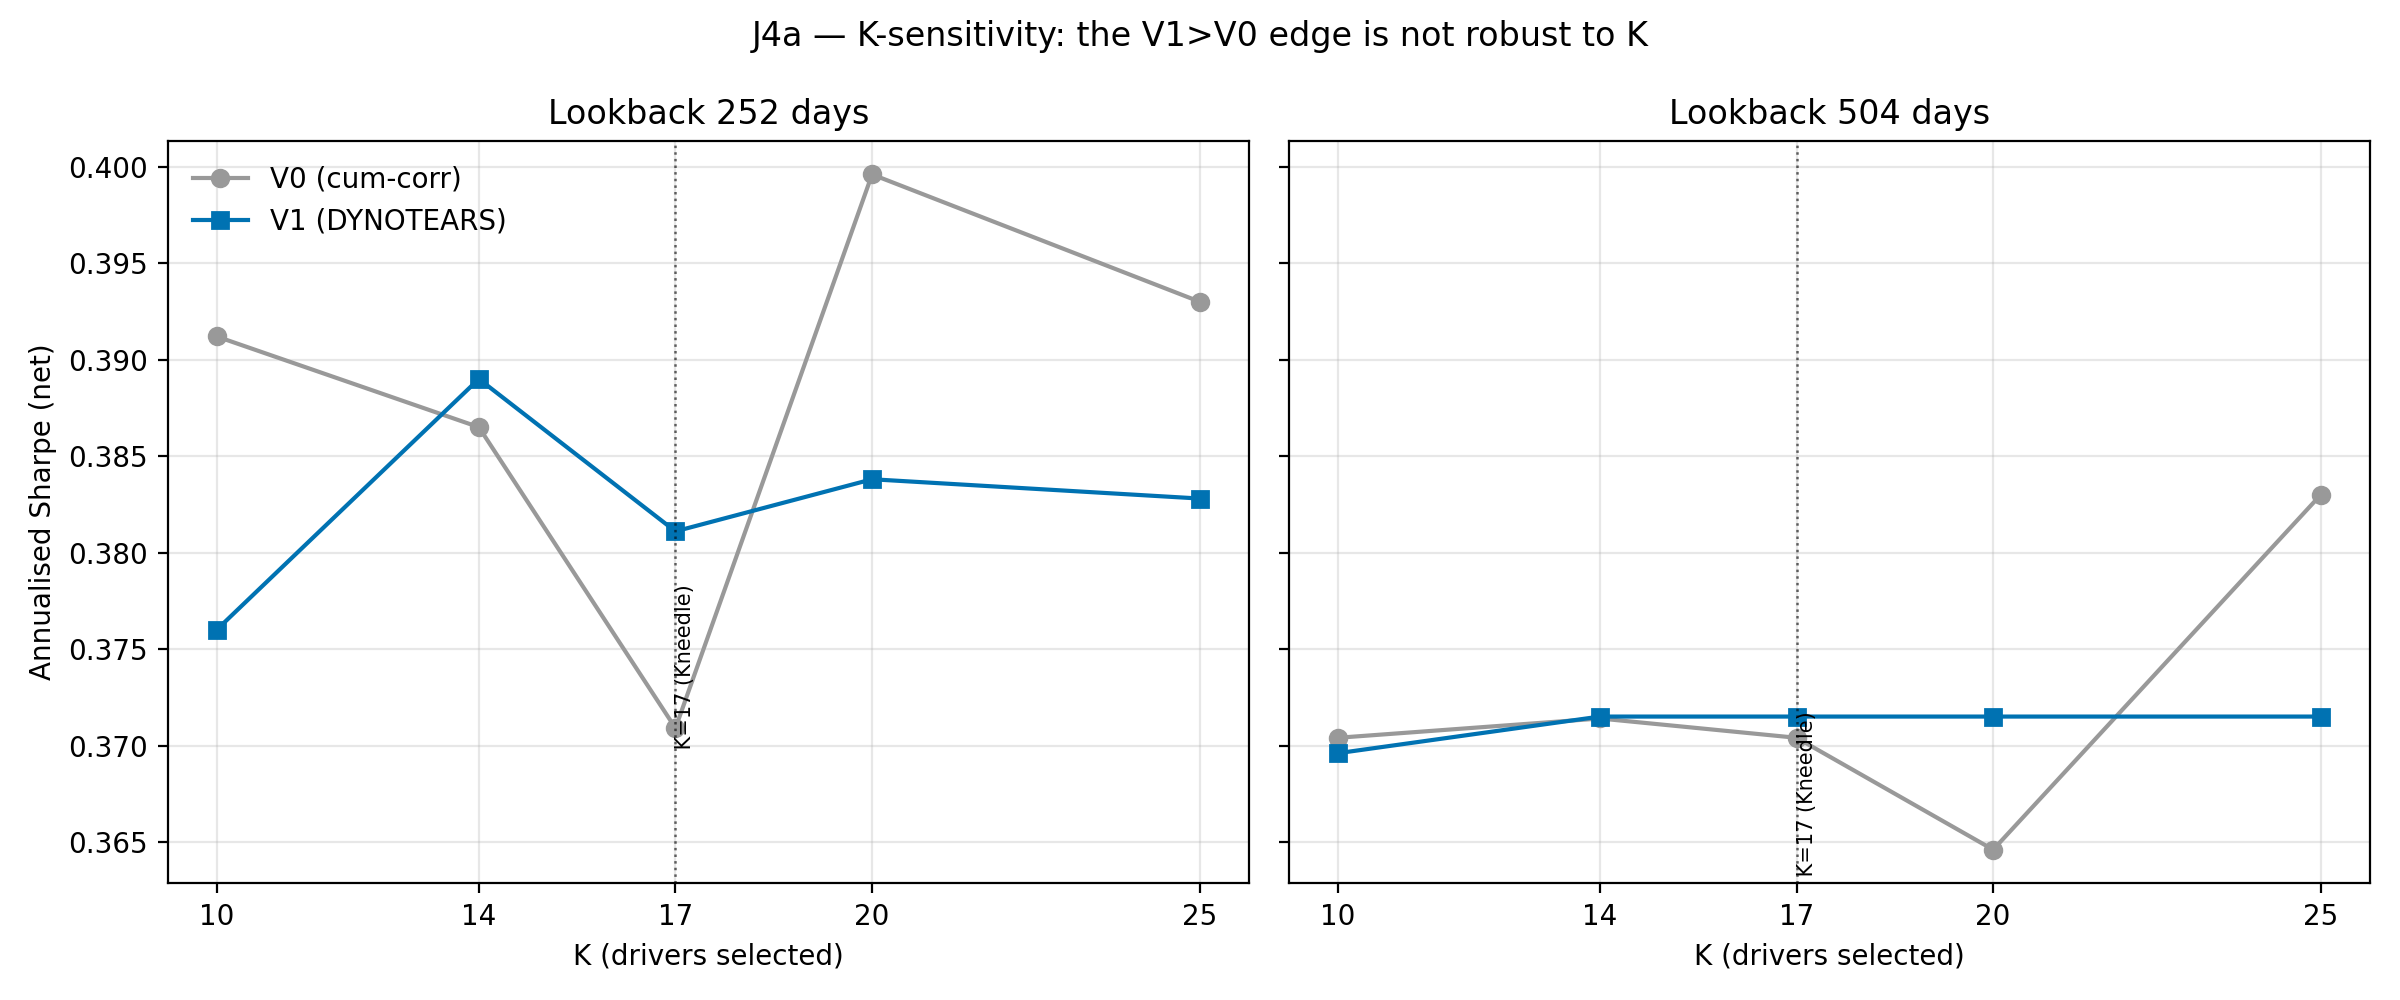
\includegraphics[width=0.97\textwidth]{figures/k_sensitivity.png}
  \caption{The driver route's $K$-fragility: net Sharpe of \hspbase{} and
    \hspcausal{}
    (DYNOTEARS) across the number of selected drivers $K$. The correlation
    selector's Sharpe varies erratically with $K$ while \hspcausal{} is
    stable, so the
    sign of their difference depends on $K$: \hspcausal{} leads at $K=14$
    and $K=17$ and trails at $K=10$, $20$ and $25$. No
    difference is significant.}
  \label{fig:ksens}
\end{figure}

\begin{figure}[tbp]
  \centering
  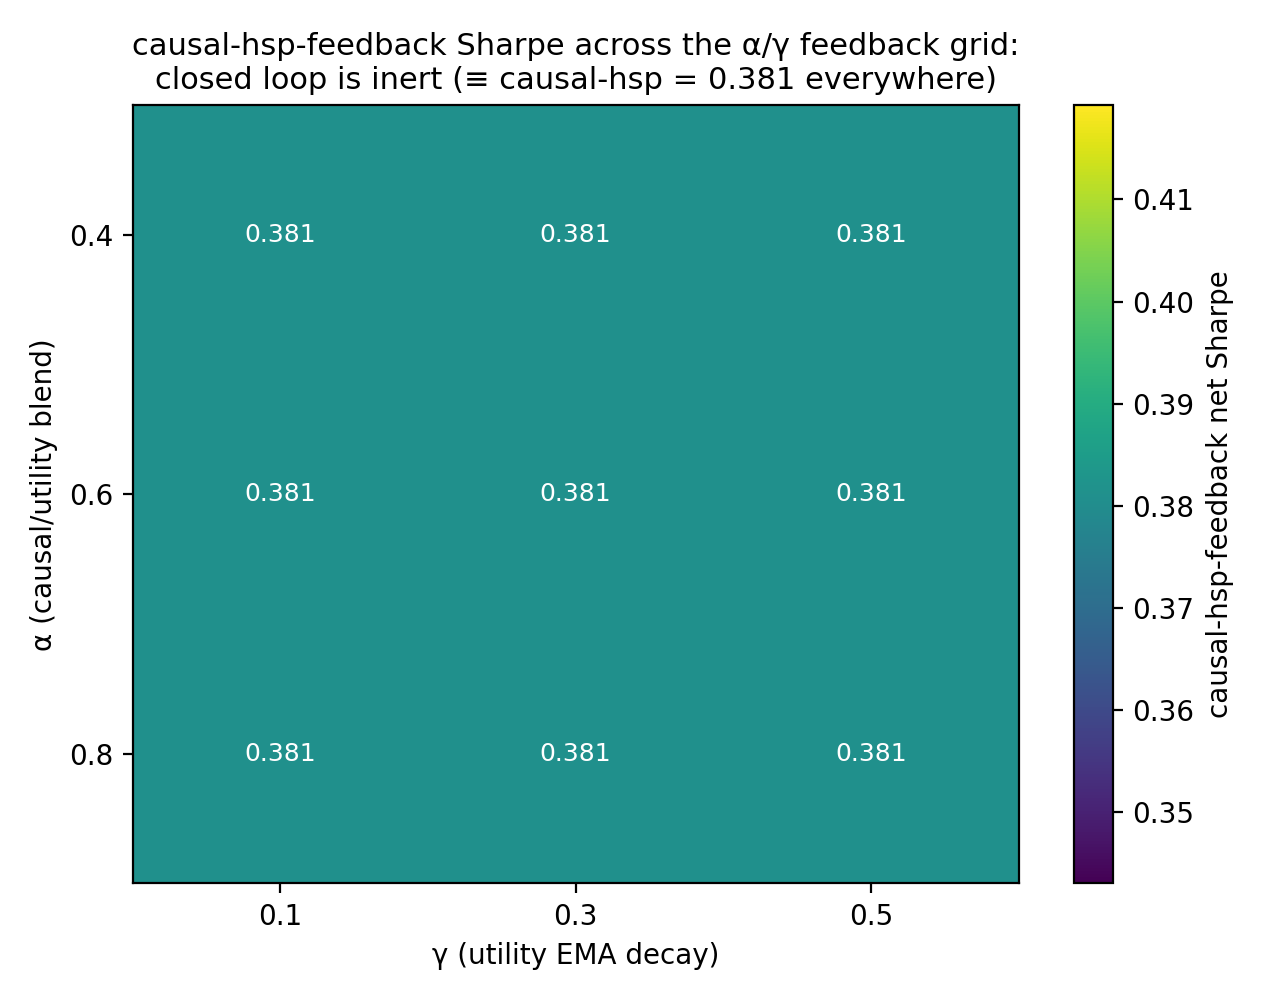
\includegraphics[width=0.7\textwidth]{figures/feedback_grid.png}
  \caption{The closed loop is inert: \hsploop{} net Sharpe across the
    $\alpha\times\gamma$ feedback grid (one-year window) is $0.381$
    everywhere, identical to open-loop \hspcausal{} to four decimals. The
    feedback
    can only re-rank within the causally-selected set, and its monthly reward
    has signal-to-noise ${\approx}\,\rsRewardSNR$.}
  \label{fig:grid}
\end{figure}

\section{The decomposition: skeleton versus orientation}
\label{sec:decomposition}

\subsection{The decomposition across estimation horizons}

Figure~\ref{fig:gradient} is the thesis's central result:
the two components of the decomposition traced across the four estimation
windows. Figure~\ref{fig:decomp} shows the per-window levels,
Table~\ref{tab:decomp} the numbers, and Figure~\ref{fig:heatmap} the full
allocator--method matrix. Three features carry the answer to the research
question. First, the
total causal-graph gain is stable: $+0.018$ to $+0.032$ (\skelsem{}) at
every
horizon, rising to $+0.036$ for \orientsem{} at two years. Second, the
skeleton contribution is hump-shaped ($-0.003$ at nine months, peaking at
$+0.022$ at the one-year convention, decaying to $+0.009$ at two years) and
never individually significant ($p \geq 0.14$). Third, the
orientation contribution is positive at every window and U-shaped ($+0.021$ at
$p=0.08$, $+0.009$ at $p=0.45$, $+0.012$ at $p=0.31$, $+0.023$ at
$p=0.048$): largest at the two extremes, smallest where the skeleton peaks,
with 11 of the 12 DYNOTEARS orientation contrasts positive across the grid
(Figure~\ref{fig:forest}). The two components are roughly complementary,
which is why the total is flat while its composition shifts. Family-wise,
Hansen's SPA over the direction-aware variants of both methods against
the shared skeleton control (\skelsamp{} on DYNOTEARS graphs, the V0$'$
replication; VARLiNGAM's variants are held to the same benchmark rather
than their own skeleton)
gives $p=\rsSpaDirWone$, $\rsSpaDirWtwo$, $\rsSpaDirWthree$ and
$\rsSpaDirWfive$ across the four windows, rejecting at the $5\%$ level
only at two years, where the pairwise effect also peaks;
Section~\ref{sec:believe-rigour} sizes that rejection.

\paragraph{Anchor-dependence of the shapes.} The contributions above are
anchored
on \skelsamp{}. Re-anchoring on \skelalt{}, the symmetrisation with the
stronger orientation-blindness guarantee (Section~\ref{sec:controls}),
changes them: the skeleton contribution becomes flat ($+0.022$, $+0.018$,
$+0.024$, $+0.019$ across the four windows) and the orientation
contribution
becomes $-0.003$/$+0.013$/$+0.006$/$+0.012$ for \skelsem{}
($-0.003$/$+0.008$/$+0.010$/$+0.016$ for \orientsem{}; point estimates,
not formally tested). The two anchors agree that orientation's increment
is positive at every window from one year out and largest at the longer
horizons; they disagree at nine months, where the symmetrisation choice
itself moves the controls by as much as the contributions do (the $+0.025$,
$p=0.013$ control-versus-control divergence reported under robustness
below). The hump and the U are therefore \skelsamp{}-anchored
descriptions; the anchor-robust findings are the flat-to-positive
skeleton gain, the long-horizon orientation increment, and the
narrowed-family rejections (Section~\ref{sec:believe-rigour}), which
land on the anchor-robust region.

\begin{figure}[tbp]
  \centering
  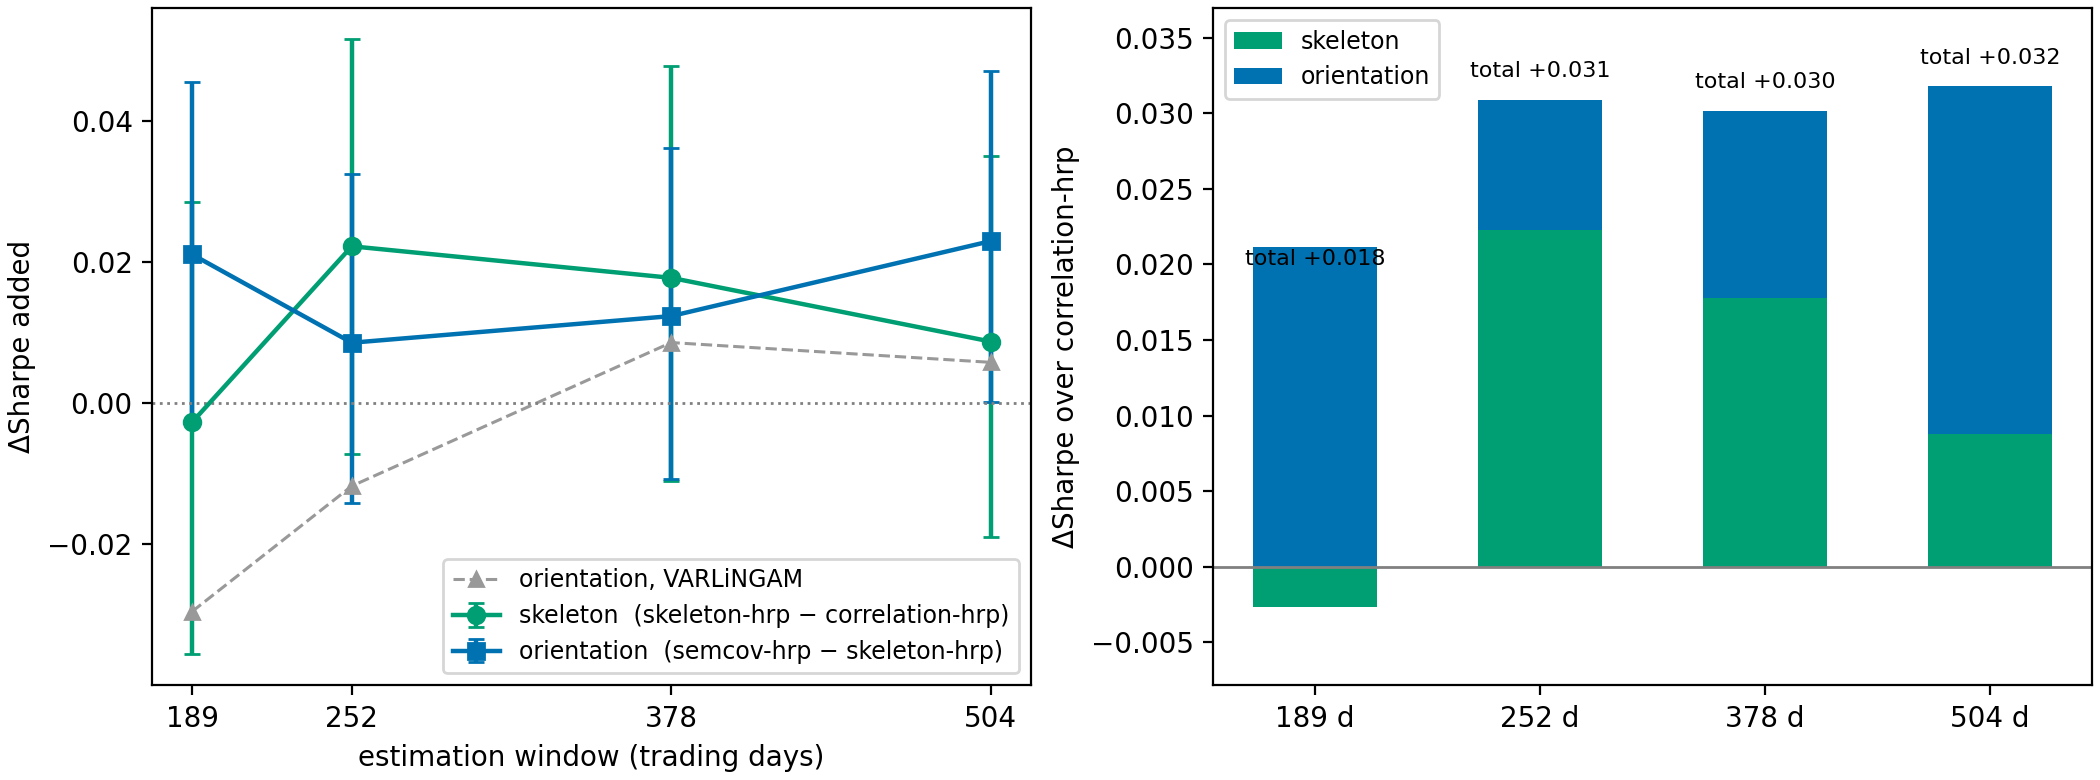
\includegraphics[width=0.99\textwidth]{figures/phase_ii_window_gradient.png}
  \caption{The central result: the two components of the decomposition as a
    function of estimation-window length (DYNOTEARS, net Sharpe). Left: the
    skeleton addition (\skelsamp{} $-$ \HRP{}, hump-shaped) and the
    orientation addition (\skelsem{} $-$ \skelsamp{}, U-shaped, positive throughout) with
    $95\%$ block-bootstrap CIs; the VARLiNGAM orientation series (grey)
    scatters around zero (mean $-0.005$), dipping below it at the
    nine-month window. Right: the same two additions stacked. The total gain
    is stable while its composition shifts, orientation contributing most
    where the sample moments feeding the control are weakest.}
  \label{fig:gradient}
\end{figure}

\begin{table}[t]
  \centering
  \caption{The decomposition (DYNOTEARS): pairwise $\Delta$Sharpe with
    Politis--Romano $p$-values at each estimation window. The total splits
    by the shared anchor: total $=$ skeleton $+$ orientation.}
  \label{tab:decomp}
  \small
  \setlength{\tabcolsep}{4pt}
  \begin{tabular}{l c c c c}
    \toprule
    & \multicolumn{4}{c}{Window (days)} \\
    \cmidrule(lr){2-5}
    Contrast & 189 & 252 & 378 & 504 \\
    \midrule
    skeleton: \skelsamp{} $-$ \HRP{} & $-0.003$ (0.85) & $+0.022$ (0.14) & $+0.018$ (0.24) & $+0.009$ (0.53) \\
    orientation, allocation step: \skelsem{} $-$ \skelsamp{}     & $+0.021$ (0.08) & $+0.009$ (0.45) & $+0.012$ (0.31) & $+0.023$ (0.048) \\
    orientation, both steps: \orientsem{} $-$ \skelsamp{}   & $+0.021$ (0.19) & $+0.003$ (0.82) & $+0.017$ (0.29) & $+0.027$ (0.057) \\
    \midrule
    total: \skelsem{} $-$ \HRP{}   & $+0.018$ (0.43) & $+0.031$ (0.15) & $+0.030$ (0.15) & $+0.032$ (0.11) \\
    total: \orientsem{} $-$ \HRP{} & $+0.019$ (0.42) & $+0.026$ (0.24) & $+0.035$ (0.10) & $+0.036$ (0.077) \\
    \bottomrule
  \end{tabular}
\end{table}

\begin{figure}[tbp]
  \centering
  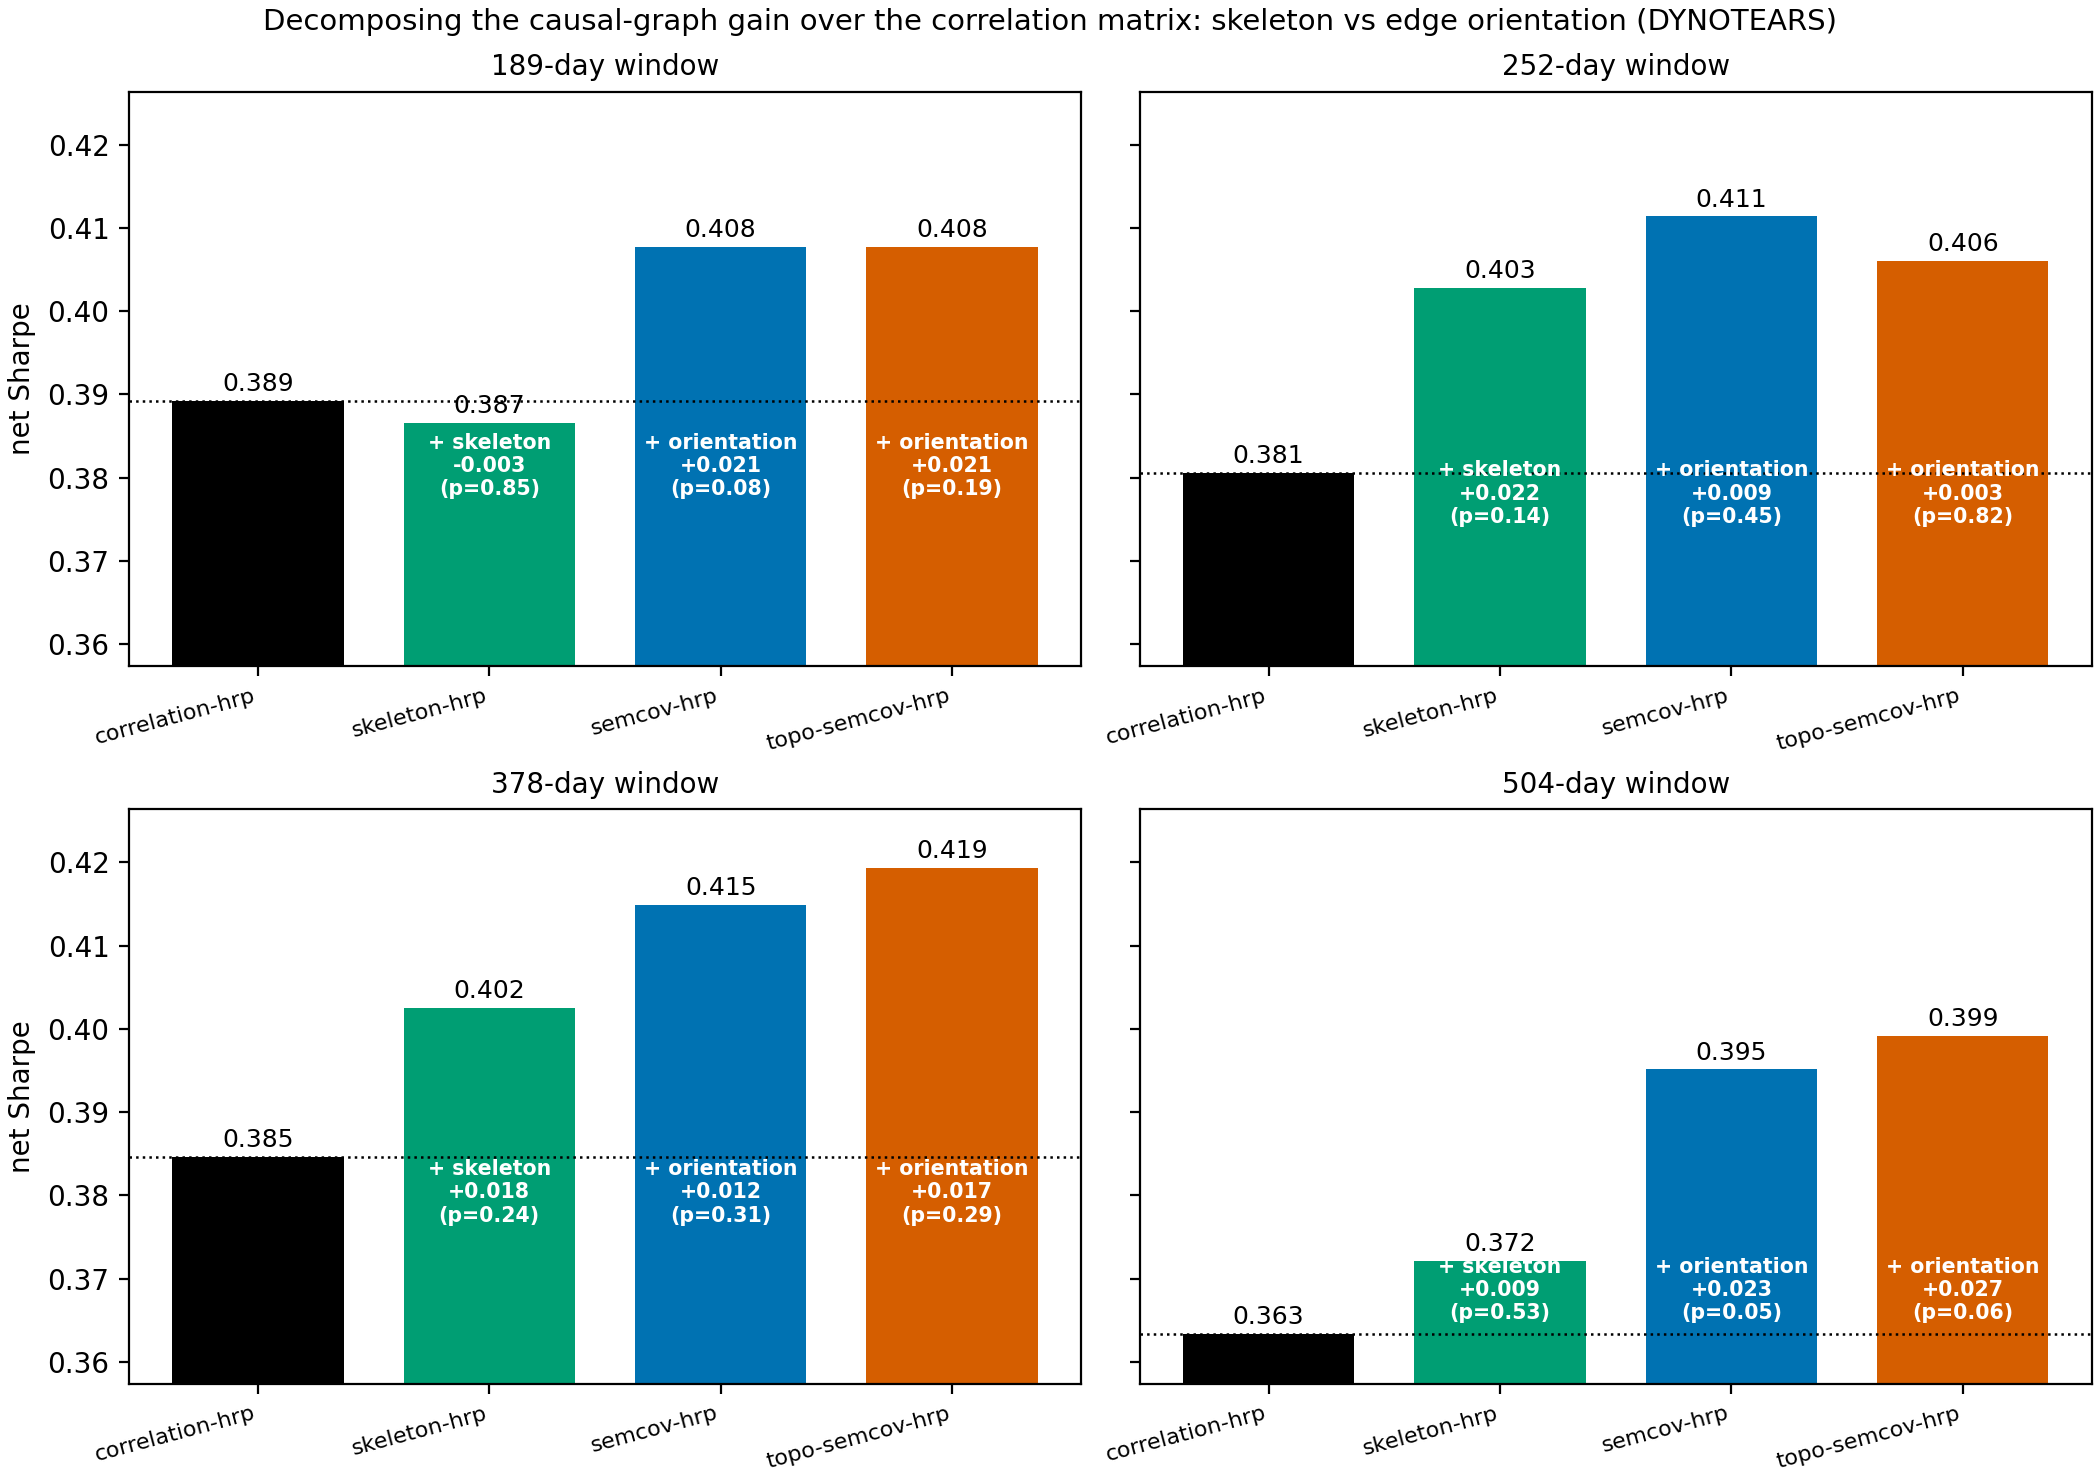
\includegraphics[width=0.99\textwidth]{figures/phase_ii_decomposition.png}
  \caption{The per-window levels behind Figure~\ref{fig:gradient}
    (DYNOTEARS graphs, net annualised Sharpe): \HRP{} $\to$ \skelsamp{}
    ($+$skeleton) $\to$ \skelsem{}/\orientsem{} ($+$orientation) at each estimation window,
    steps annotated with the pairwise bootstrap $\Delta$ and $p$-value.
    Section~\ref{sec:believe-rigour} adjudicates these steps family-wise.}
  \label{fig:decomp}
\end{figure}

\begin{figure}[tbp]
  \centering
  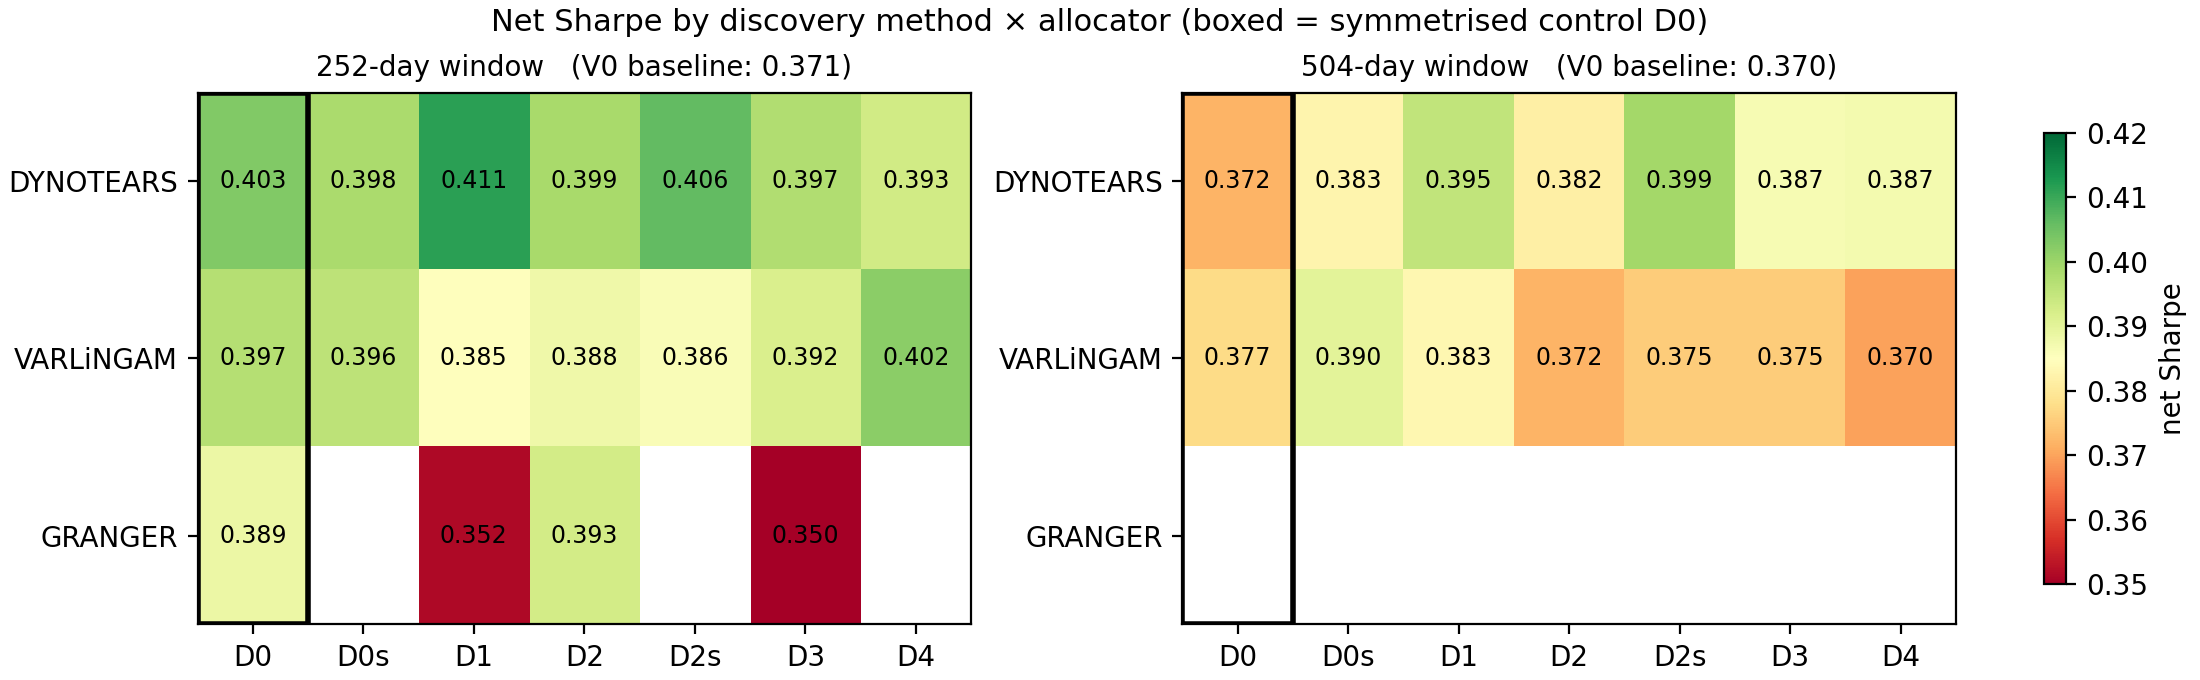
\includegraphics[width=0.99\textwidth]{figures/phase_ii_heatmap.png}
  \caption{Net Sharpe by discovery method $\times$ allocator at the four
    windows (boxed column: the symmetrised control \skelsamp{}; panel titles carry
    the \HRP{} baseline). The DYNOTEARS orientation-aware cells (\skelsem{},
    \orientsem{}) are strong at every window (\orientsem{} at 378 days,
    0.419, is the
    study-wide best), while the VARLiNGAM rows show no orientation effect
    anywhere.}
  \label{fig:heatmap}
\end{figure}

\begin{figure}[tbp]
  \centering
  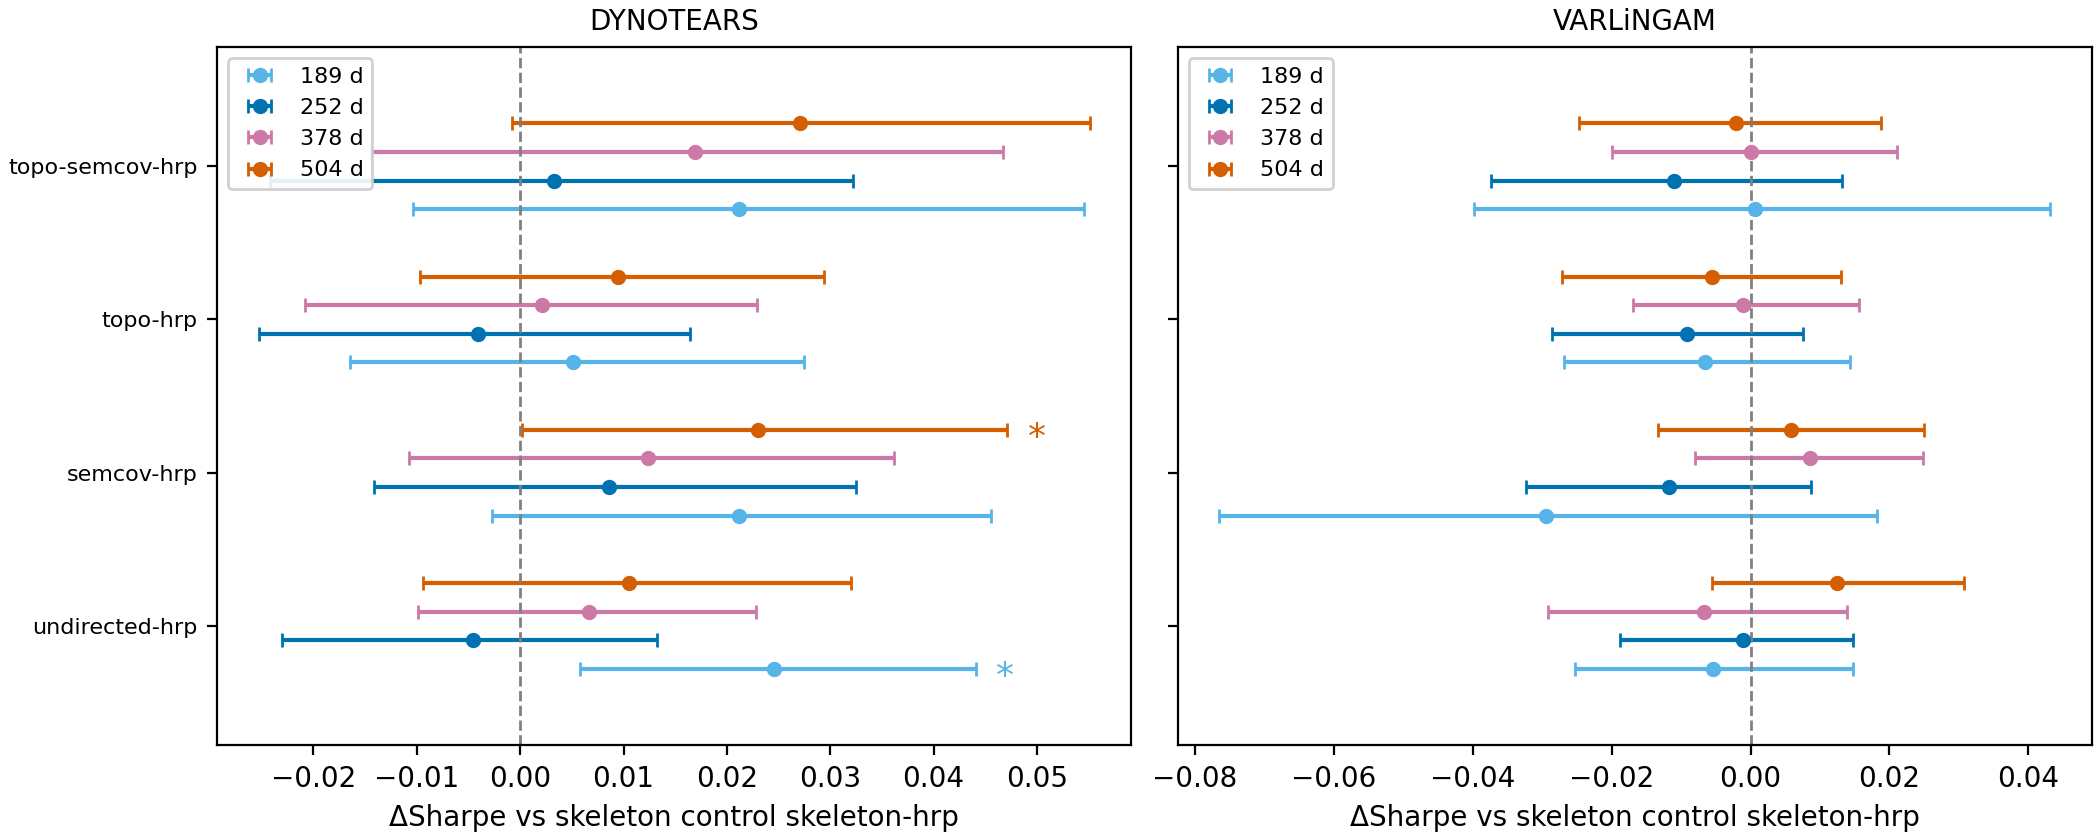
\includegraphics[width=0.99\textwidth]{figures/phase_ii_forest.png}
  \caption{The fixed-graph orientation effect: $\Delta$Sharpe of each
    orientation-aware allocator against the skeleton control \skelsamp{} at all four
    windows, with $95\%$ block-bootstrap CIs ($\ast$: $p<0.05$). Eleven of
    twelve DYNOTEARS contrasts are positive (\skelsem{} starred at two years); the
    VARLiNGAM contrasts scatter around zero (4/12 positive). The starred
    \skelalt{} cell at the nine-month window is a control-versus-control
    divergence, discussed in the text.}
  \label{fig:forest}
\end{figure}

\subsection{What orientation contributes}
\label{sec:orientation-role}

Orientation contributes robustness to the estimation horizon rather than
level. The skeleton
allocator's performance is window-fragile ($0.372$--$0.403$ across the four
windows, and below the control at nine months); \skelsem{}
($0.395$--$0.415$) and
\orientsem{} ($0.399$--$0.419$) are strong everywhere
(Figure~\ref{fig:nav} shows the
one-year NAV paths). The U-shape of Figure~\ref{fig:gradient} indicates
when orientation pays: when the sample moments
feeding the allocator are least reliable. At 189 days the sample covariance
is estimated from barely $1.9$ observations per asset (noise); at 504 days
it averages across regimes it should distinguish (staleness); and at the
one-year window, where the estimation literature puts the
noise--staleness optimum and where the skeleton's own contribution peaks,
orientation adds least. $\Sigma_{\mathrm{SEM}}$, built from the
contemporaneous graph and its shock variances, substitutes structure
for sample-moment quality at both ends of that trade-off. On this reading,
the SEM covariance acts as a regulariser of the allocation step rather
than a source of extra return; the controls at the end of this
subsection identify which of its properties does the regularising, and
the answer is not direction. Two qualifications bound the mechanism. First,
the window moves the graph and the sample moments together (both are
estimated on the same lookback), so the gradient cannot by itself
separate moment degradation from graph degradation; the stability of the
discovered graphs across windows (density $6.3$--$6.9\%$ at every
horizon; Section~\ref{sec:asset-graph}) supports, but does not prove, the
reading that the moments degrade faster. Second, the nine-month arm of
the U is anchor-dependent (Section~\ref{sec:decomposition}), so the
regulariser mechanism is asserted with confidence only on its
long-horizon arm, where both anchors agree.

\paragraph{An alternative explanation, tested directly.} The
contrast $\skelsem{}-\skelsamp{}$ compares the SEM-implied covariance
against the sample covariance, and $\Sigma_{\mathrm{SEM}}$ differs from
the sample covariance in more ways than direction: it is a structured
estimator (fewer effective parameters, shrinkage-like in character), and
its independent-shock assumption strips out the common market component.
Either property is achievable with no graph at all, so a sceptic could
read the covariance-channel gain as generic shrinkage or as
de-factoring. I test both directly, with the interpretation of every
possible outcome written down and committed before either control was
run (Section~\ref{sec:believe}): the skeleton allocator's clustering is
kept fixed and its sample covariance is replaced by (i) a Ledoit--Wolf
shrunk covariance \cite{ledoitwolf2004} and (ii) a de-factored covariance (each asset
regressed on the window's equal-weight market return, allocation on the
residual covariance), neither of which sees an edge direction. The
shrinkage account fails: the Ledoit--Wolf control sits below the plain
skeleton at every window ($\rsDlwSharpeWone$, $\rsDlwSharpe$,
$\rsDlwSharpeWthree$, $\rsDlwSharpeWfive$ across the four horizons), and
\skelsem{} beats it by $+0.018$ to $+0.042$ ($p=0.05$ at two years, its
strongest window; $p \geq 0.08$ elsewhere).
The de-factoring account succeeds: the de-factored control
($\rsDdfSharpeWone$, $\rsDdfSharpe$, $\rsDdfSharpeWthree$,
$\rsDdfSharpeWfive$) reproduces the covariance channel at every window,
leaving a residual \skelsem{}-minus-control of $-0.011$ to $+0.004$
($p \geq 0.5$ throughout). Following the reading committed in advance,
the
covariance-channel gain is not attributed to directional content: the
operative ingredient of $\Sigma_{\mathrm{SEM}}$ is its independent-shock
assumption, which removes the common market component, and that removal
needs no graph. What survives for the orientations is a weaker,
conditional role. DYNOTEARS magnitudes recover the full de-factoring
benefit without damaging it, whereas the identical construction on
VARLiNGAM graphs, equally structured and equally de-factored, yields
nothing, and its magnitude-degraded ridge-Granger version collapses (both
shown in the discovery-method comparison of the next subsection).
Trustworthy edge magnitudes are therefore necessary for the construction
to work; but the working ingredient is the de-factoring, not the
direction of the edges.

\paragraph{The skeleton channel, given the same treatment.} The
covariance controls discipline the orientation channel; symmetry demands
the same scepticism of the skeleton channel. Its gain over \HRP{}
($+0.022$ at the one-year window) could in principle be reproduced by
any sparse conditional-dependence structure of the same density, with no
discovery at all. A third control tests this directly, with
interpretations again committed before it was run
(\texttt{PREDICTIONS\_SKELETON\_CONTROL.md}): \skelsamp{}'s construction
with the discovered skeleton replaced by a thresholded
partial-correlation matrix (Ledoit--Wolf precision, largest-magnitude
cells kept, density-matched by nonzero-cell count to the paired graph,
which enters only through that scalar). The
graph-free skeleton fails to reproduce the channel exactly where it
pays: at the
one-year window it earns $\rsDpcSharpe$ against the discovered
skeleton's $0.403$, a residual of $+0.025$ ($p=0.008$), and its own gain
over
the correlation control is zero there ($-0.003$, $p=0.86$). At the
other three windows the two skeletons are statistically
indistinguishable (residuals within $\pm 0.004$, $p \geq 0.69$), which
is where the skeleton
channel pays little anyway. Following that reading, the
skeleton channel's paying region is attributed to the discovered
skeleton itself. The mechanism story is therefore asymmetric in an
informative way: the orientation channel's covariance gain needs no
graph (de-factoring reproduces it), while the skeleton channel's
one-year gain does.

\begin{figure}[tbp]
  \centering
  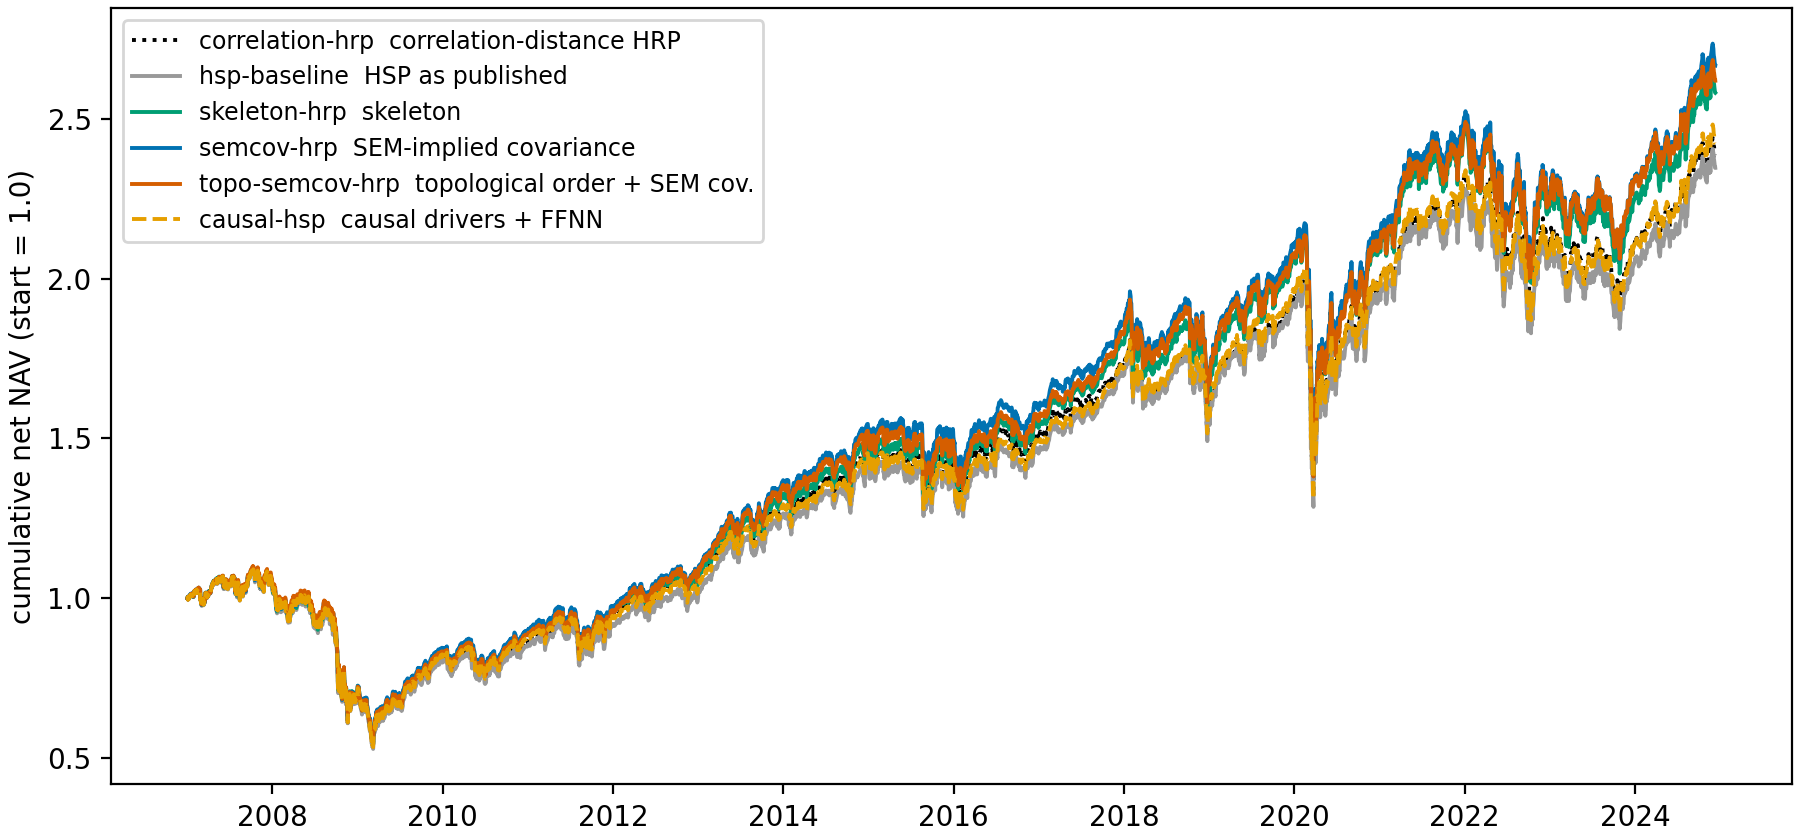
\includegraphics[width=0.99\textwidth]{figures/phase_ii_nav.png}
  \caption{Cumulative net NAV, one-year window: the correlation control, the
    \hspbase{}, the skeleton \skelsamp{}, the orientation-aware \skelsem{}
    and \orientsem{}, and
    the driver route \hspcausal{}. All variants absorb the full ${\approx}50\%$ GFC
    drawdown; the study concerns relative allocation quality, not
    drawdown avoidance.}
  \label{fig:nav}
\end{figure}

\subsection{Robustness to design parameters}

\paragraph{Sparsity ($\tau$).} Thresholding the graph at
$\tau\in\{0,0.01,0.05,0.10\}$ leaves the treatment flat-to-better
(\orientsamp{}:
$0.399\to0.402$ at the heaviest threshold) while the
skeleton control drifts down ($0.403\to0.394$; Table~\ref{tab:tau}), so
the orientation-aware
allocators are not artefacts of the regularisation threshold. These sweep
differences are point estimates; they were not formally tested.

\paragraph{Costs and turnover.} The covariance-channel increment is
cost-invariant in point estimates: \skelsem{}$-$\skelsamp{} at two years
moves from $+0.022$ to $+0.025$ as
costs rise from 0 to 20\,bps (differences on unrounded series;
Table~\ref{tab:cost}), because \skelsem{}'s turnover ($0.102$
one-way per
rebalance) is below the control's ($0.112$). The claim does not extend
to the ordering route at short windows: \orientsem{} carries the
family's highest turnover ($0.140$), and its one-year increment erodes
from $+0.004$ at zero cost to $0.000$ at 20\,bps, while its two-year
increment survives the sweep. The covariance channel does not win by
trading less and is not eroded by trading more; the ordering channel at
one year is.

\paragraph{Discovery method.} Under VARLiNGAM graphs the orientation effect
is absent at all four windows (4 of 12 contrasts positive, mean $-0.005$;
Figure~\ref{fig:forest}, right, and the grey series of
Figure~\ref{fig:gradient}). The decomposition is therefore
\emph{method-dependent}: DYNOTEARS' jointly-optimised, acyclicity-constrained
$W$ supports orientation-aware allocation where VARLiNGAM's ICA-ordered
$B_0$ does not. This is consistent with VARLiNGAM's identification
weakening as
residuals Gaussianise over longer windows and, at the nine-month window,
with its unpruned $B_0$ saturating in the thin-sample regime (density
$32\%$ against DYNOTEARS' stable $6$--$7\%$;
Section~\ref{sec:asset-graph}),
so its short-window graphs carry little usable orientation signal either.
A DYNOTEARS graph supplies two things at once, the direction of each
edge and a fitted magnitude for it, so its cells alone cannot show which
of the two the orientation effect consumes; the ridge-Granger control
separates them, preserving a usable ordering while degrading the
magnitudes. It thereby localises where inside
the orientation the value sits: causal-ordered bisection survives on its
graphs (\orientsamp{} $=0.393$ vs DYNOTEARS' $0.399$) while the
SEM-covariance
allocator collapses (\skelsem{} $=0.352$; gap $-0.060$,
$p=0.11$). A ridge-VAR coefficient matrix carries a serviceable
ordering but not structural effect sizes, so the dissociation indicates
that orientation's contribution does not lie in merely knowing which way
the
arrows point (an ordering survives even a one-lag ridge regression)
but in edge magnitudes trustworthy enough to propagate shocks, the
ingredient only the jointly-optimised DYNOTEARS fit supplies. This is a
refinement of the answer to the research question, not a separate benchmark: ``orientation''
pays through its weighted, propagatable form.

\paragraph{The controls disagree at the shortest window.} At 189 days the
two orientation-blind symmetrisations diverge: \skelalt{} beats
\skelsamp{} by $+0.025$
($p=0.013$), the strongest control-versus-control divergence in the
study. The implication is that at the shortest
window
the choice of symmetrisation matters as much as orientation itself,
so the nine-month skeleton and orientation contributions carry an extra layer of
estimator uncertainty that the anchored decomposition cannot remove; the
nine-month column is read with that caveat throughout.

\paragraph{A second family member (HERC).} Chapter~\ref{chap:background}'s
family-wide framing is an interface claim: any hierarchical allocator
clustering on a symmetric matrix discards orientation, whatever its
tree-reading rule. Whether the \emph{measured} decomposition generalises
across tree-reading rules is a separate, empirical question, and I test
it on a second member with interpretations committed before any cell
was run (\texttt{PREDICTIONS\_HERC.md}): a full-recursion Hierarchical
Equal Risk Contribution allocator \cite{raffinot2018herc}, identical to
the HRP family in clustering stage and cluster-risk measure, but
descending the dendrogram's actual topology instead of bisecting the
leaf ordering. Three cells mirror the decomposition (correlation
control, skeleton member on \skelsamp{}'s distance, orientation member
on $\Sigma_{\mathrm{SEM}}$; Appendix~\ref{app:tables}). The outcome is
the mixed reading, and it bounds the generalisation
informatively. The orientation channel's sign carries: $+0.119$,
$+0.131$, $+0.018$ and $+0.092$ across the four windows (unadjusted
bootstrap $p = 0.03$, $0.03$, $0.81$, $0.21$), positive everywhere, as
under HRP. The skeleton channel's does not ($-0.203$, $-0.193$,
$+0.011$, $-0.040$; $p \geq 0.16$), and the whole HERC family sits well
below its HRP counterparts (control $0.245$--$0.325$). The mechanical
reading is an interface interaction: under the house single-linkage
pattern the dendrogram is deeply chained, and walking its topology
compounds roughly a hundred sequential budget splits, which HRP's
balanced bisection of the ordering never does; the embedding-distance
tree is evidently more chained still at the shorter windows. The
decomposition's magnitudes are therefore allocator-specific: what
generalises to this second member is orientation's sign, not the
skeleton's contribution, and the family-wide claim is retained only in
its interface form. All twelve HERC cells join the deflation universe
and neither SPA family; Raffinot's cluster-cut variant, which prunes
the walk, is the natural next member to test.

\subsection{Regime dependence}
\label{sec:regimes}

The prior-verification result (Section~\ref{sec:discovery-run}) showed
edge
assignment matters most in stress windows, motivating the hypothesis
that orientation-aware allocation would add most value in crises. The
regime-conditional analysis contradicts this (Figure~\ref{fig:regime};
Table~\ref{tab:regime-full} gives every variant, including the graph-blind
controls, so within-regime treatment-versus-control differences can be
read directly): at
the
one-year window the orientation-aware allocators' edge over \hspbase{}
(the shared weakest baseline, chosen so every variant is visible on one
scale)
concentrates
in the bottom VIX quintile ($+0.22$/$+0.25$ Sharpe for
\skelsem{}/\orientsem{}) and is
approximately zero (\skelsem{}) to negative (\orientsem{}) in the top
quintile, while in NBER
recessions the skeleton allocator is the strongest and \skelsem{} adds
nothing. These regime-conditional figures are descriptive; no formal
regime-level test was run, and conditional Sharpe levels are mechanically
inflated in the calm regime (the volatility denominator conditions on
low-VIX days), so only cross-strategy differences within a regime are
read. A
plausible reading is that in stress, correlations rise toward one and any
structure, causal or correlational, is swamped by the common factor,
while in calm markets cross-sectional causal heterogeneity is the signal.
Whatever the mechanism, the hypothesis as stated was wrong and is
reported as such, an outcome that Howard et al.'s stable-regime centrality
alpha (Section~\ref{sec:howard-theme}) had anticipated.

\begin{figure}[tbp]
  \centering
  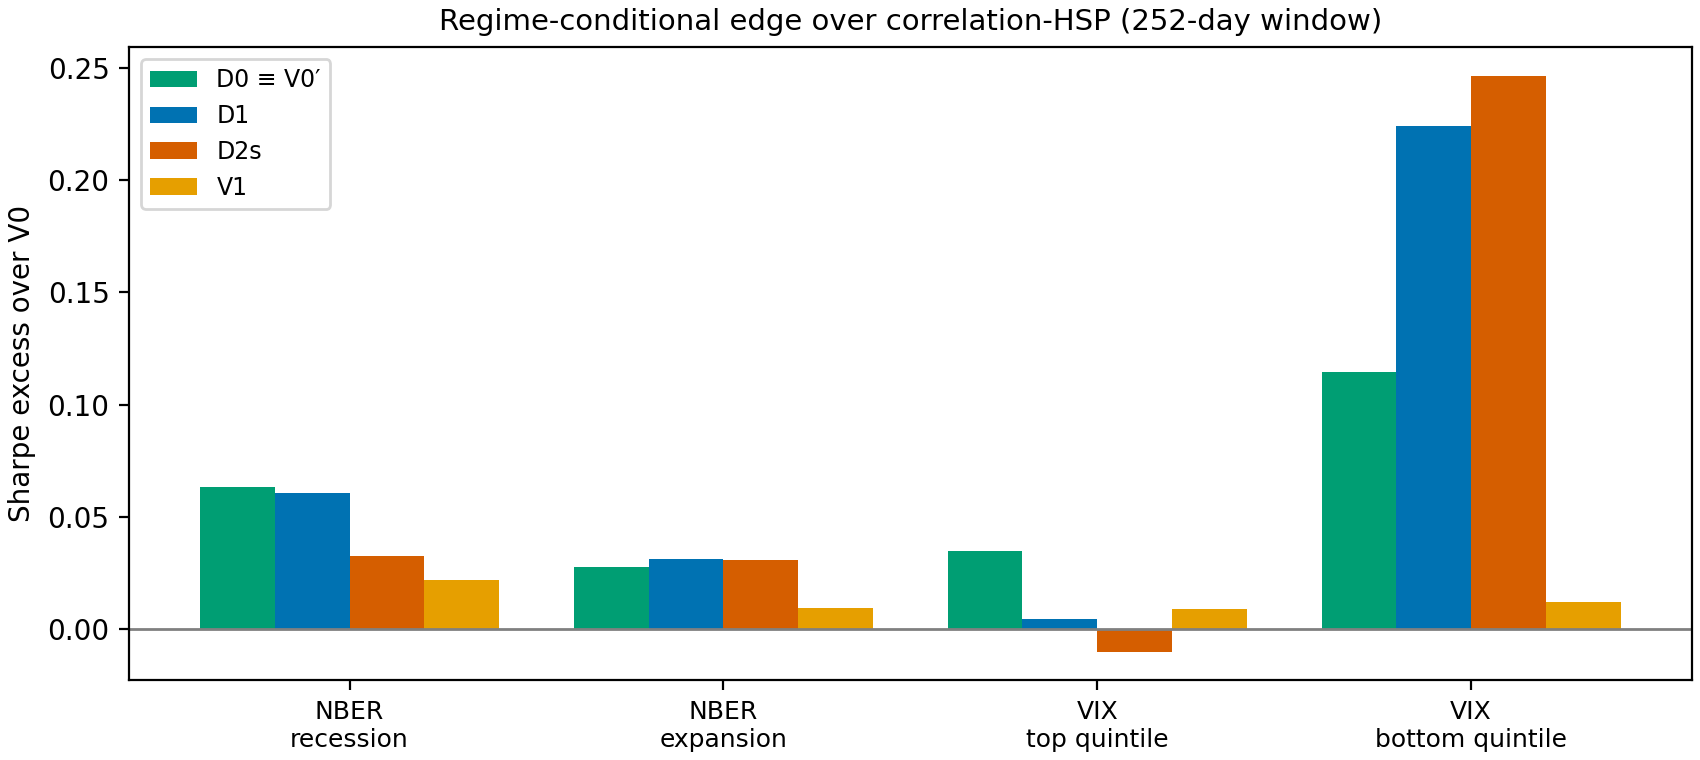
\includegraphics[width=0.9\textwidth]{figures/phase_ii_regime.png}
  \caption{Regime-conditional Sharpe excess over \hspbase{} (one-year window).
    The
    orientation-aware edge concentrates in the VIX bottom quintile (calm
    markets), not in stress: the stress hypothesis is rejected.}
  \label{fig:regime}
\end{figure}

\section{Multiplicity-aware adjudication}
\label{sec:believe-rigour}

% Numbers in this section come from _generated/robust_stats.tex, regenerated
% by `python -m scripts.robust_stats --phase-ii` over all evaluated bundles.

\paragraph{Non-normality and selection bias (PSR/DSR).} Every headline
allocator's Probabilistic Sharpe ratio (the probability its true Sharpe
exceeds zero given the sample's higher moments) is high (\HRP{}
$\rsCorrPSR$, \skelsamp{} $\rsVprimePSR$, \skelsem{} $\rsDonePSR$ at
one year), so the
levels are not fat-tail artefacts. Deflating against the best Sharpe
expected from \rsNtrials\ no-skill trials, the study's highest Deflated
Sharpe ratio belongs to \orientsem{} at the 18-month window
($\rsDtwosDSRWthree$), followed by the direction-free de-factored
control ($\rsDdfDSRWthree$) and \skelsem{} ($\rsDoneDSRWthree$), against
the control's $\rsCorrDSR$ and the skeleton's
$\rsVprimeDSR$; the top of the deflation table is filled by the
orientation-aware cells and the de-factored control that mimics them,
itself consistent with the mechanism finding of
Section~\ref{sec:orientation-role}. The ordering of the decomposition survives deflation;
how much of its statistical separation survives is what the family-wise
tests size next.

\paragraph{Family-wise comparisons (RC/SPA).} Four SPA families
adjudicate the claims with the search priced in, and every window-level
test is run twice: first over the full allocator grid (all
seven graph-consuming allocators of the experiment plan, both discovery
methods), then over the
narrower family the report's taxonomy defines (the $2\times2$ crossing
plus the second symmetrisation control). The narrowing was fixed only
after the four-window results had been seen, so the full grid's
numbers are the primary ones and the narrowed family's are reported
second and labelled as such. Two of the families are single tests:
\textbf{(i)} causal-structure strategies vs \hspbase{} at one
year gives $p=\rsSpaConsistent$, significant, but as Section~\ref{sec:r1}
showed, substantially a verdict on \hspbase{}'s machinery; and
\textbf{(iv)} the Chapter-\ref{chap:sensitivity} allocator family
against \hspbase{} gives
$p=\rsSpaDvarPre$ over the full grid and $\rsSpaDvar$ narrowed,
significant under neither. The two window-level families, \textbf{(ii)}
the causal family vs the \HRP{} control and \textbf{(iii)} the
orientation-aware variants vs the shared skeleton control (\skelsamp{}
on DYNOTEARS graphs; Section~\ref{sec:decomposition}), are tabulated in
Table~\ref{tab:spa}, whose final column prices the search across
strategies \emph{and} the four estimation windows in a single pooled
family against the one-year control.

\begin{table}[t]
  \centering
  \caption{Hansen's SPA consistent $p$-values by family, window and
    grid. ``Pooled'' runs one SPA whose candidate set is the union of
    the family's cells at all four windows against the family's one-year
    control, so it prices the strategy search and the window search
    jointly. Bold: $p<0.05$.}
  \label{tab:spa}
  \small
  \begin{tabular}{l l c c c c c}
    \toprule
    Family & Grid & 189 & 252 & 378 & 504 & Pooled \\
    \midrule
    (ii) vs \HRP{}      & full     & $\rsSpaSkelWonePre$ & $\rsSpaSkelWtwoPre$ & $\rsSpaSkelWthreePre$ & $\rsSpaSkelWfivePre$ & $\rsSpaSkelPooledPre$ \\
    (ii) vs \HRP{}      & narrowed & $\rsSpaSkelWone$ & $\rsSpaSkelWtwo$ & $\mathbf{\rsSpaSkelWthree}$ & $\mathbf{\rsSpaSkelWfive}$ & $\rsSpaSkelPooled$ \\
    (iii) vs \skelsamp{} & full     & $\rsSpaDirWonePre$ & $\rsSpaDirWtwoPre$ & $\rsSpaDirWthreePre$ & $\rsSpaDirWfivePre$ & $\rsSpaDirPooledPre$ \\
    (iii) vs \skelsamp{} & narrowed & $\rsSpaDirWone$ & $\rsSpaDirWtwo$ & $\rsSpaDirWthree$ & $\mathbf{\rsSpaDirWfive}$ & $\rsSpaDirPooled$ \\
    \bottomrule
  \end{tabular}
\end{table}

In sum: under the full grid the
only rejection is family (i), against the weak incumbent anchor. Every
window-level rejection quoted in this report
($p=\rsSpaSkelWthree$--$\rsSpaDirWfive$, the longest horizons of
families (ii) and (iii)) exists only under the post-hoc narrowing.
The pooled column completes the multiplicity accounting on the axis the
per-window tests leave unpriced, and it is decisive in the deflationary
direction: once the window search is priced alongside the strategy
search, nothing rejects for either family, under either grid
($p=\rsSpaSkelPooled$ for the narrowed causal family,
$\rsSpaDirPooled$ for the narrowed orientation family). The
window-level rejections are therefore read as
suggestive rather than established: they coincide with, and add
modestly to, the sign-consistent point estimates, but the
full grid's family-wise evidence does not reject anywhere on the
window grid, and the jointly-priced test does not reject at all.

\paragraph{The Model Confidence Set.} The $90\%$ MCS over the
\rsMcsUniverse\ distinct one-year strategies retains \rsMcsSize\ of them,
eliminating only \rsMcsExcluded. This is best read as a statement about
power, not a vindication of everything retained: with seventeen highly
correlated long-only variants whose Sharpes span $0.35$--$0.41$, the
equivalence test can only discriminate against the strategy that loses
consistently, \hspbase{}. The MCS confirms its
inferiority and otherwise declines to rank the causal family, including
declining to separate treatments from controls.

\paragraph{The seed audit.}
\label{sec:seed-audit}
Re-running the committed driver-route configuration (\hspcausal{}, one-year
window,
$K{=}17$) under \rsSeedN\ neural-network seeds (discovery cached, so the
initialisation is the only varying ingredient) moves its net
Sharpe across $[\rsSeedMin, \rsSeedMax]$ (median $\rsSeedMedian$;
Figure~\ref{fig:seed}). The range ($\rsSeedRange$) is more than twice the
$+0.010$ edge the arm claims over its own baseline, and the committed value
sits at the $\rsSeedPct$th percentile of its own seed distribution: at
the unluckiest seed the edge all but vanishes. This quantifies, on this
pipeline, the concern that neural sensitivity-based results are fragile to
undisclosed seed choices, and it is the strongest argument for the
deterministic graph-based family: at the one-year window the audit ran
at, every DYNOTEARS-graph member of the
reported family sits above the seed
cloud's maximum (the headline allocators \skelsamp{}, \skelsem{} and
\orientsem{} comfortably so)
and produces identical results on every run
(Table~\ref{tab:seed-full} gives the full audit).

\begin{figure}[tbp]
  \centering
  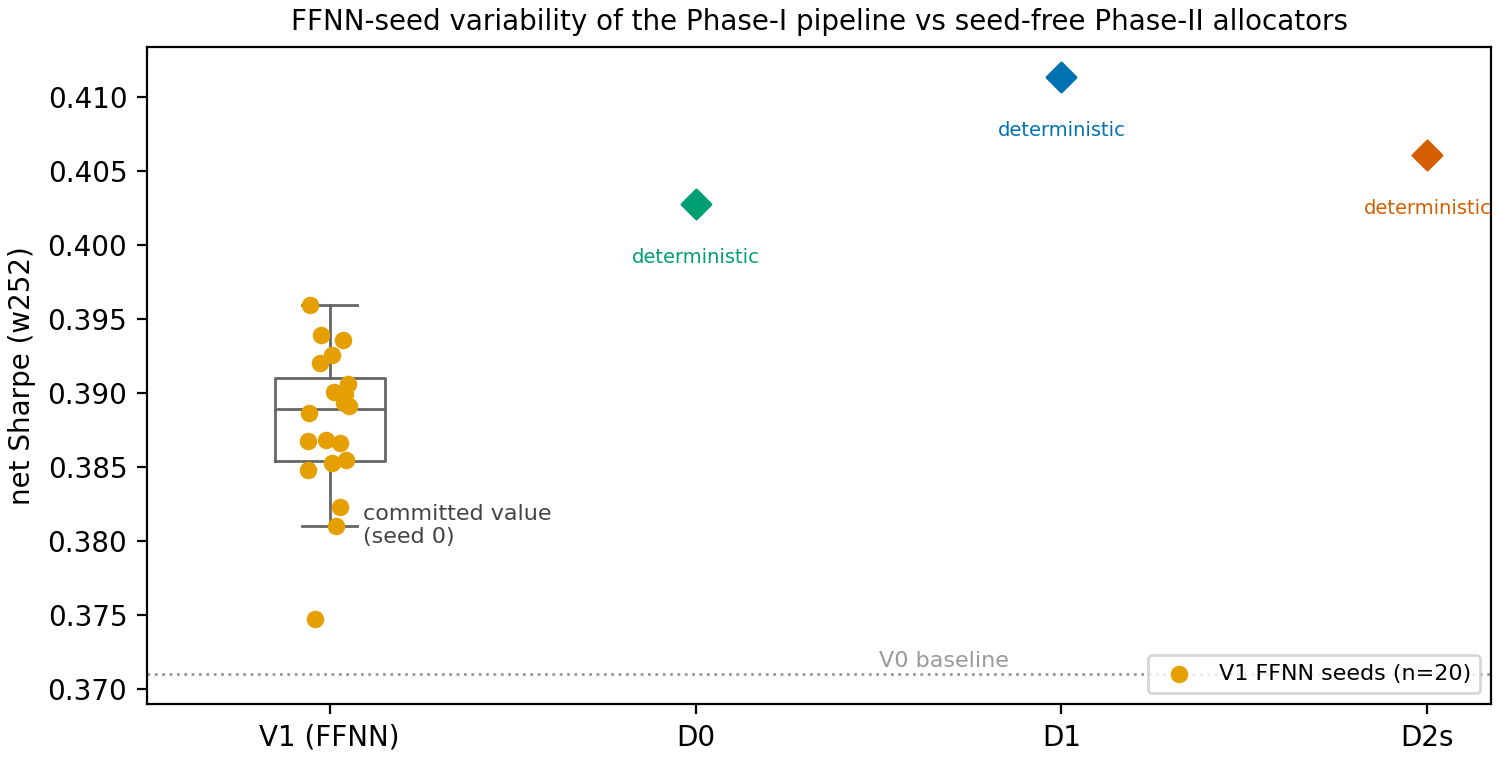
\includegraphics[width=0.85\textwidth]{figures/phase_ii_seed.png}
  \caption{The seed audit: net Sharpe of the driver route \hspcausal{} across
    \rsSeedN\ network seeds (one-year window), against the deterministic
    graph-based allocators. The seed range exceeds \hspcausal{}'s claimed edge over
    its baseline; the graph-based allocators shown sit above the seed-cloud
    maximum.}
  \label{fig:seed}
\end{figure}

\paragraph{Verdict on the research question, with uncertainty stated.} The decomposition's
point estimates are clear and internally consistent: a stable total
gain whose composition shifts with the horizon (skeleton hump-shaped and
peaking at the one-year convention, orientation positive at every window
and largest at the extremes), with the orientation-aware allocators
topping the study-wide DSR table. Its statistical support is
modest and reported at its estimated size: 36 of 40
graph-versus-correlation cells
positive; one pairwise-significant orientation cell among twelve
($p=0.048$) and one suggestive one ($p=0.08$); no family-wise rejection
anywhere under the full grid; under the post-hoc narrowed
family only, marginal rejections confined to the longest horizons
(Requirement 1 at 18 months and two years,
$p=\rsSpaSkelWthree$ and $\rsSpaSkelWfive$; orientation at two years,
$p=\rsSpaDirWfive$), coinciding with the peaks of the point
estimates; and no rejection for either family once the pooled test
prices the window search alongside the strategy search
(Table~\ref{tab:spa}). The mechanism controls of Section~\ref{sec:orientation-role}
bound what the orientation edge means: its covariance channel is
reproduced by a graph-free de-factored covariance, so the defensible
gain is one of robustness, not of directional information as such. The
skeleton control sharpens this into an asymmetric verdict: the skeleton
channel's one-year gain is not reproduced by a graph-free skeleton of
matched density, so what the discovery machinery itself earns is
concentrated in the skeleton at the conventional window. The
largest defensible claim is therefore conditional and modest: if one
replaces the correlation matrix with a DYNOTEARS graph, the skeleton pays
only near the conventional one-year window; keeping the orientations
costs nothing and improves robustness to the estimation-horizon choice,
though the same improvement is available from de-factoring the
covariance with no graph at all; and the long-horizon edge is suggestive
under the narrowed family, unsupported under the full grid, and
dissolves when the window search is priced jointly with the strategy
search.

\section{An out-of-sample slice}
\label{sec:oos}

Every result so far shares the 2007--2024 panel, and
Section~\ref{sec:believe} discloses three design choices that were
informed by results on that panel. A deflation correction is not a
substitute for out-of-sample replication, so I ran one: the identical
harness, universe, cost model and DYNOTEARS configuration on
2025-01 to 2026-07, a span that did not exist when the design was
fixed. The protocol and the interpretation of every possible outcome
were committed before any out-of-sample price was fetched
(\texttt{PREDICTIONS\_OOS.md}), including this constraint, stated in
advance: 19 monthly rebalances (399 trading days) put the standard
error of an annualised Sharpe near $0.8$ and of the pairwise contrasts
near $0.08$, so \emph{the slice is a sign and magnitude check on the
point estimates, and no $p$-value computed on it counts as evidence in
either direction}. Two protocol notes: CRSP daily data ends 2024-12-31,
so the slice's prices come from Yahoo Finance (the source switch is
confined to the slice and disclosed here), and all 99 names remained
listed throughout it.

\begin{table}[t]
  \centering
  \caption{Out-of-sample contrasts (net $\Delta$Sharpe,
    2025-01 to 2026-07, point estimates only). Every sign the
    protocol specified in advance is consistent with the in-sample
    decomposition;
    at this sample length the contrast standard errors are roughly
    $0.08$, so magnitudes are not interpreted.}
  \label{tab:oos}
  \small
  \begin{tabular}{l c c c c}
    \toprule
    & \multicolumn{4}{c}{Window (days)} \\
    \cmidrule(lr){2-5}
    Contrast & 189 & 252 & 378 & 504 \\
    \midrule
    skeleton: \skelsamp{} $-$ \HRP{}          & $+0.057$ & $+0.096$ & $+0.102$ & $+0.144$ \\
    orientation: \skelsem{} $-$ \skelsamp{}   & $+0.035$ & $+0.076$ & $+0.121$ & $+0.073$ \\
    orientation: \orientsem{} $-$ \skelsamp{} & $-0.042$ & $+0.009$ & $+0.088$ & $+0.095$ \\
    total: \skelsem{} $-$ \HRP{}              & $+0.091$ & $+0.172$ & $+0.223$ & $+0.217$ \\
    residual: \skelsem{} $-$ de-factored      & $-0.011$ & $-0.009$ & $-0.004$ & $+0.020$ \\
    \bottomrule
  \end{tabular}
\end{table}

The outcome matches the consistency reading
(Table~\ref{tab:oos}). The total gain is positive at all four windows,
the \skelsem{} orientation increment is positive at all four, and
\orientsem{}'s is positive from one year out with its only negative
cell at nine months, the window whose in-sample contributions already
carried the anchor-dependence caveat. The skeleton contribution,
hump-shaped in sample, is positive at every window here. The mechanism
reading also carries at point-estimate level: the graph-free
de-factored control again sits within $0.011$ of \skelsem{} at three
windows (and $0.020$ below it at two years), so out of sample too the
covariance channel behaves like de-factoring. Two honesty notes bound
this. The slice is a strong bull market (control Sharpe levels of
$0.78$--$0.92$), so the absolute magnitudes are inflated relative to
the 2007--2024 panel and are not compared to it; and with contrast
standard errors near $0.08$, agreement of signs is all the slice can
certify. Within those limits, every specified sign
came back consistent with the in-sample decomposition, on data that did
not exist when the design, the family and the question were fixed.

\section{Threats to validity}
\label{sec:believe}

\paragraph{Effect sizes sit near the detection floor.} The decomposition's
components are $0.01$--$0.03$ Sharpe over 18 years, against a full-sample
Sharpe standard error of ${\approx}\,\rsSharpeSEFull$ (Lo's
approximation on the $\sim$4{,}500-day sample). The pairwise contrasts
are far more precise, because the strategies are highly
correlated and the bootstrap differences the joint panel: the
block-bootstrap standard error of the total contrast
(\skelsem{}$-$\HRP{} at one year) is $\rsContrastSETotal$ and of the
orientation contrast (\orientsem{}$-$\skelsamp{}) $\rsContrastSEOrient$.
Those standard errors put numbers on ``underpowered'': at $5\%$ size and
$80\%$ power the one-sided minimum detectable effects are
${\approx}\,\rsContrastMDETotal$ and ${\approx}\,\rsContrastMDEOrient$
net Sharpe respectively, roughly twice the observed $+0.031$ total and
$+0.023$ orientation increments. The design could therefore only have
certified effects about double the size actually observed, and that cuts
both ways: the
rejections that do occur are marginal and narrowed-family only
($p=\rsSpaSkelWthree$--$\rsSpaDirWfive$), and the absence of rejection at
the shorter horizons is not evidence of absence. At the pairwise level, one
$p=0.048$ cell among twelve orientation contrasts is close to what
multiplicity predicts under the null, which is why no single cell is
claimed as a discovery. The orientation effect earns its standing not from
any single
cell but from the sign-consistency of the contribution across all four
windows and both orientation-aware treatments against the primary anchor,
positive from one year out under the alternative anchor as well
(Section~\ref{sec:decomposition}), with the narrowed-family rejections
landing on that anchor-robust region.

\paragraph{Forking-paths risk.} Three design choices were informed by
earlier results, and this section is their record. The choice of question
was informed by the first phase's results. The window grid reached its
four-horizon form in two stages: the conventional 252- and 504-day windows
were evaluated first, and the 189- and 378-day windows were added when the
initial results suggested a composition shift that a two-point design
cannot distinguish from noise. Three disciplines bound the associated
risk: the added windows were run symmetrically (every allocator, both
methods, all cells reported); the deflation universe covers all
\rsNtrials\ configurations ever evaluated, both phases, all windows; and
the headline reading (orientation positive everywhere, largest at the
extremes) would have been weakened, and reported as such, had the added
windows come back inconsistent. The narrowed-family rejections inherit
the risk asymmetrically: the strongest (Requirement 1 at 378 days,
$p=\rsSpaSkelWthree$)
sits on an added window, while the two-year rejections
($p=\rsSpaSkelWfive$, $\rsSpaDirWfive$) sit on windows evaluated from the
start, which bounds the concern for them.

The third informed choice is the family itself, and it is the most
consequential. The plan's grid contained seven allocators,
including the structural-shock risk parity on $\Sigma_{\mathrm{SEM}}$
and the co-ancestry-distance variant; the narrowing to the five
allocators of the two-entry-point taxonomy of
Chapter~\ref{chap:sensitivity} was made after the four-window results
had been seen. The taxonomy is a principled reason for the smaller
family (the thesis question is about HRP's two entry points, and those
two arms enter the graph elsewhere), but the timing means the narrowed
family's rejections cannot be read as
confirmatory, and it is exactly the choice
the significance turns on: every family-wise number is therefore
reported for both families in Section~\ref{sec:believe-rigour}, and
under the full grid nothing on the window axis rejects
($p=\rsSpaSkelWthreePre$, $\rsSpaSkelWfivePre$, $\rsSpaDirWfivePre$
where the narrowed family gives $\rsSpaSkelWthree$, $\rsSpaSkelWfive$,
$\rsSpaDirWfive$). The two excluded arms stay in the deflation universe,
and their results are directionally consistent with the family they were
excluded from (above the control in all sixteen of their cells, both
discovery methods and all four windows, by $+0.002$ to $+0.024$;
Appendix~\ref{app:tables}), so the exclusion is not results-driven in
direction, but the reader should weigh the narrowed-family rejections
with the timing in view. Separately, the two mechanism controls of
Section~\ref{sec:orientation-role} were added after this chapter's
results were first drafted, in response to the objection that
$\Sigma_{\mathrm{SEM}}$'s gain might be generic; their interpretations
were written down and committed before either control was run, and they
join the deflation universe but neither family.

\paragraph{Single asset class, one universe, approximated index.} Everything
here concerns long-only allocation within ${\sim}100$ US large-caps; every
variant absorbs the full ${\approx}50\%$ GFC drawdown. Whether the
decomposition transfers to universes with richer exogenous structure
(multi-asset, credit, commodities) is untested. The top-by-market-cap
approximation of the S\&P~100, the fixed snapshot-union universe (whose
membership is partly settled by market caps realised later in the
sample) and the absence of delisting returns
(Section~\ref{sec:asset-graph}) carry
mild residual survivorship and look-ahead effects. Their sign is
favourable, but they are shared by every allocator on the same panel, so
they inflate the absolute levels rather than the pairwise contrasts the
thesis is about; quantifying them with a point-in-time universe is left
to future work.

\paragraph{Method-dependence is a caveat on the mechanism.} The orientation
effect exists under DYNOTEARS graphs only. Until a second discovery method
reproduces it, the safest interpretation is ``DYNOTEARS' contemporaneous
structure supports orientation-aware allocation'', not ``causal orientation
in markets is allocatively valuable''.

\paragraph{What the evidence supports, and does not.} It supports: the
graph's consistent, modest improvement over the correlation matrix (36 of
40 cells); the horizon-dependent composition of that gain (skeleton
hump-shaped, orientation U-shaped and positive throughout); the
regulariser role of the SEM covariance, now identified by the direct
controls as de-factoring rather than directional content; a
narrowed-family edge over the stronger controls at the longest horizons,
marginal and reported as such; and the dominance of
deterministic graph-based allocation over the seed-unstable,
feedback-inert driver route.
It does not support: any family-wise rejection under the full
allocator grid; family-wise significance near the one-year
convention under either family; attribution of the covariance-channel
gain to edge direction; any orientation effect under VARLiNGAM; or the
stress hypothesis. That profile, precise point estimates whose
suggestive family-wise support appears only under a post-hoc narrowing,
and whose leading mechanism a direction-free control reproduces,
is the finding.
